\documentclass[border=4pt,crop=true]{standalone}
\usepackage{pgfplots}
\pgfplotsset{compat=1.18}

% $|H|/(R_f/R) = (omega/omega_0)/sqrt(1+(omega/omega_0)^2), omega_0=1/(RC), R_f=R
% Ideal differentiator same norm: omega/omega_0 for omega<<omega_0

\begin{document}
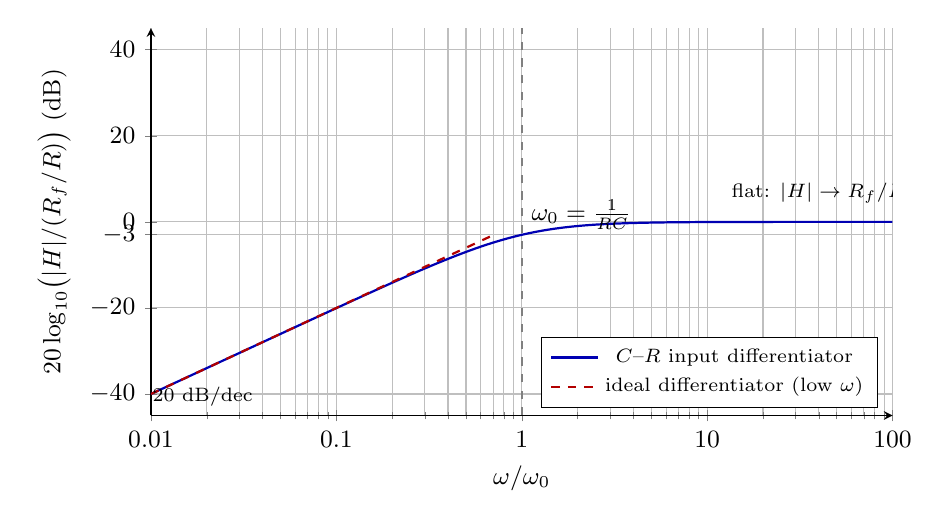
\begin{tikzpicture}
  \begin{axis}[
    width=11cm,
    height=6.5cm,
    xmode=log,
    xmin=1e-2,
    xmax=1e2,
    ymin=-45,
    ymax=45,
    axis lines=left,
    xlabel={$\omega/\omega_0$},
    ylabel={$20\log_{10}\bigl(|H|/(R_f/R)\bigr)$ (dB)},
    xtick={1e-2,1e-1,1,1e1,1e2},
    xticklabels={$0.01$,$0.1$,$1$,$10$,$100$},
    ytick={-40,-20,-3,0,20,40},
    grid=both,
    minor tick num=1,
    tick label style={font=\small},
    label style={font=\small},
    every axis plot/.append style={thick},
    legend style={font=\scriptsize,at={(0.98,0.02)},anchor=south east},
  ]
    \addplot[blue!70!black,domain=1e-2:1e2,samples=300]
      {20*ln(x)/ln(10) - 10*ln(1+x^2)/ln(10)};
    \addplot[red!70!black,dashed,domain=1e-2:0.7,samples=200]
      {20*ln(x)/ln(10)};
    \addplot[gray,dashed] coordinates {(1,-45) (1,45)};
    \node[anchor=south west,font=\small] at (axis cs:1,-4)
      {$\omega_0=\frac{1}{RC}$};
    \node[anchor=north east,font=\scriptsize] at (axis cs:0.04,-36)
      {$+20$ dB/dec};
    \node[anchor=south west,font=\scriptsize] at (axis cs:12,2)
      {flat: $|H|\to R_f/R$};
    \legend{$C$--$R$ input differentiator, ideal differentiator (low $\omega$)}
  \end{axis}
\end{tikzpicture}
\end{document}
